% xcolor and define colors -------------------------
\usepackage{xcolor}

% https://www.viget.com/articles/color-contrast/
\definecolor{purple}{HTML}{5601A4}
\definecolor{navy}{HTML}{0D3D56}
\definecolor{ruby}{HTML}{9a2515}
\definecolor{alice}{HTML}{107895}
\definecolor{daisy}{HTML}{EBC944}
\definecolor{coral}{HTML}{F26D21}
\definecolor{kelly}{HTML}{829356}
\definecolor{cranberry}{HTML}{E64173}
\definecolor{jet}{HTML}{131516}
\definecolor{asher}{HTML}{555F61}
\definecolor{slate}{HTML}{314F4F}

% Mixtape Sessions
\definecolor{picton-blue}{HTML}{00b7ff}
\definecolor{violet-red}{HTML}{ff3881}
\definecolor{sun}{HTML}{ffaf18}
\definecolor{electric-violet}{HTML}{871EFF}

\newcommand\pictonBlue[1]{{\color{picton-blue}#1}}
\newcommand\sun[1]{{\color{sun}#1}}
\newcommand\electricViolet[1]{{\color{electric-violet}#1}}
\newcommand\violetRed[1]{{\color{violet-red}#1}}

\newcommand\bgPictonBlue[1]{{\colorbox{picton-blue!20!white}{#1}}}
\newcommand\bgSun[1]{{\colorbox{sun!20!white}{#1}}}
\newcommand\bgElectricViolet[1]{{\colorbox{electric-violet!20!white}{#1}}}
\newcommand\bgVioletRed[1]{{\colorbox{violet-red!20!white}{#1}}}

\def\code#1{\texttt{#1}}

% Main theme colors
\definecolor{accent}{HTML}{00b7ff}
\definecolor{accent2}{HTML}{871EFF}
\definecolor{gray100}{HTML}{f3f4f6}
\definecolor{gray800}{HTML}{1F292D}


% Beamer Options -------------------------------------

% Background
\setbeamercolor{background canvas}{bg = white}

% Change text margins
\setbeamersize{text margin left = 15pt, text margin right = 15pt} 

% \alert
\setbeamercolor{alerted text}{fg = accent2}

% Frame title
\setbeamercolor{frametitle}{bg = white, fg = jet}
\setbeamercolor{framesubtitle}{bg = white, fg = accent}
\setbeamerfont{framesubtitle}{size = \small, shape = \itshape}

% Block
\setbeamercolor{block title}{fg = white, bg = accent2}
\setbeamercolor{block body}{fg = gray800, bg = gray100}

% Title page
\setbeamercolor{title}{fg = gray800}
\setbeamercolor{subtitle}{fg = accent}

%% Custom \maketitle and \titlepage
\setbeamertemplate{title page}
{
    %\begin{centering}
        \vspace{20mm}
        {\Large \usebeamerfont{title}\usebeamercolor[fg]{title}\inserttitle}\\
        {\large \itshape \usebeamerfont{subtitle}\usebeamercolor[fg]{subtitle}\insertsubtitle}\\ \vspace{10mm}
        {\insertauthor}\\
        {\color{asher}\small{\insertdate}}\\
    %\end{centering}
}

% Table of Contents
\setbeamercolor{section in toc}{fg = accent!70!jet}
\setbeamercolor{subsection in toc}{fg = jet}

% Button 
\setbeamercolor{button}{bg = accent}

% Remove navigation symbols
\setbeamertemplate{navigation symbols}{}

% Table and Figure captions
\setbeamercolor{caption}{fg=jet!70!white}
\setbeamercolor{caption name}{fg=jet}
\setbeamerfont{caption name}{shape = \itshape}

% Bullet points

%% Fix spacing between items
\let\olditemize=\itemize 
\let\endolditemize=\enditemize 
\renewenvironment{itemize}{\vspace{0.25em}\olditemize \itemsep0.25em}{\endolditemize}

%% Fix left-margins
\settowidth{\leftmargini}{\usebeamertemplate{itemize item}}
\addtolength{\leftmargini}{\labelsep}

%% enumerate item color
\setbeamercolor{enumerate item}{fg = accent}
\setbeamerfont{enumerate item}{size = \small}
\setbeamertemplate{enumerate item}{\insertenumlabel.}

%% itemize
\setbeamercolor{itemize item}{fg = accent!70!white}
\setbeamerfont{itemize item}{size = \small}
\setbeamertemplate{itemize item}[circle]

%% right arrow for subitems
\setbeamercolor{itemize subitem}{fg = accent!60!white}
\setbeamerfont{itemize subitem}{size = \small}
\setbeamertemplate{itemize subitem}{$\rightarrow$}

\setbeamertemplate{itemize subsubitem}[square]
\setbeamercolor{itemize subsubitem}{fg = jet}
\setbeamerfont{itemize subsubitem}{size = \small}








% Links ----------------------------------------------

\usepackage{hyperref}
\hypersetup{
  colorlinks = true,
  linkcolor = accent2,
  filecolor = accent2,
  urlcolor = accent2,
  citecolor = accent2,
}


% Line spacing --------------------------------------
\usepackage{setspace}
\setstretch{1.35}


% \begin{columns} -----------------------------------
\usepackage{multicol}


% Fonts ---------------------------------------------
% Beamer Option to use custom fonts
\usefonttheme{professionalfonts}

% \usepackage[utopia, smallerops, varg]{newtxmath}
% \usepackage{utopia}
\usepackage[sfdefault,light]{roboto}

% Small adjustments to text kerning
\usepackage{microtype}



% Remove annoying over-full box warnings -----------
\vfuzz2pt 
\hfuzz2pt


% Table of Contents with Sections
\setbeamerfont{myTOC}{series=\bfseries, size=\Large}
\AtBeginSection[]{
        \frame{
            \frametitle{Roadmap}
            \tableofcontents[current]   
        }
    }


% Tables -------------------------------------------
% Tables too big
% \begin{adjustbox}{width = 1.2\textwidth, center}
\usepackage{adjustbox}
\usepackage{array}
\usepackage{threeparttable, booktabs, adjustbox}
    
% Fix \input with tables
% \input fails when \\ is at end of external .tex file
\makeatletter
\let\input\@@input
\makeatother

% Tables too narrow
% \begin{tabularx}{\linewidth}{cols}
% col-types: X - center, L - left, R -right
% Relative scale: >{\hsize=.8\hsize}X/L/R
\usepackage{tabularx}
\newcolumntype{L}{>{\raggedright\arraybackslash}X}
\newcolumntype{R}{>{\raggedleft\arraybackslash}X}
\newcolumntype{C}{>{\centering\arraybackslash}X}

% Figures

% \imageframe{img_name} -----------------------------
% from https://github.com/mattjetwell/cousteau
\newcommand{\imageframe}[1]{%
    \begin{frame}[plain]
        \begin{tikzpicture}[remember picture, overlay]
            \node[at = (current page.center), xshift = 0cm] (cover) {%
                \includegraphics[keepaspectratio, width=\paperwidth, height=\paperheight]{#1}
            };
        \end{tikzpicture}
    \end{frame}%
}

% subfigures
\usepackage{subfigure}


% Highlight slide -----------------------------------
% \begin{transitionframe} Text \end{transitionframe}
% from paulgp's beamer tips
\newenvironment{transitionframe}{
    \setbeamercolor{background canvas}{bg=accent!40!black}
    \begin{frame}\color{accent!10!white}\LARGE\centering
}{
    \end{frame}
}


% Table Highlighting --------------------------------
% Create top-left and bottom-right markets in tabular cells with a unique matching id and these commands will outline those cells
\usepackage[beamer,customcolors]{hf-tikz}
\usetikzlibrary{calc}
\usetikzlibrary{fit,shapes.misc}

% To set the hypothesis highlighting boxes red.
\newcommand\marktopleft[1]{%
    \tikz[overlay,remember picture] 
        \node (marker-#1-a) at (0,1.5ex) {};%
}
\newcommand\markbottomright[1]{%
    \tikz[overlay,remember picture] 
        \node (marker-#1-b) at (0,0) {};%
    \tikz[accent!80!jet, ultra thick, overlay, remember picture, inner sep=4pt]
        \node[draw, rectangle, fit=(marker-#1-a.center) (marker-#1-b.center)] {};%
}


% DAGS ----------------------------------------------
\usepackage{tikz}
\usetikzlibrary{shapes,decorations,arrows,calc,arrows.meta,fit,positioning}
% Tikz settings optimized for causal graphs.
\tikzset{
    -Latex,auto,node distance =1 cm and 1 cm,semithick,
    state/.style ={ellipse, draw, minimum width = 0.7 cm},
    point/.style = {circle, draw, inner sep=0.04cm,fill,node contents={}},
    bidirected/.style={Latex-Latex,dashed},
    el/.style = {inner sep=2pt, align=left, sloped}
}


% Beamer tricks -------------------------------------
% Make \pause work in align environments
\makeatletter
\renewrobustcmd{\beamer@@pause}[1][]{%
  \unless\ifmeasuring@%
  \ifblank{#1}%
    {\stepcounter{beamerpauses}}%
    {\setcounter{beamerpauses}{#1}}%
  \onslide<\value{beamerpauses}->\relax%
  \fi%
}
\makeatother



% \usepackage{slashbox}
\title{Lecture 3: Generalized Method of Moments}
\author{Chris Conlon }
\institute{NYU Stern }

\date{\today}

\begin{document}
\maketitle



\section{Testing}

\begin{frame}{Testing with MLE}
Before we discuss testing under GMM, let's look at testing under MLE.
\begin{itemize}
\item Helpful to define the \alert{likelihood ratio}
\begin{align*}
LR \equiv -2 \cdot \ln \left[ \frac{\mathcal{L}(\theta_1 | x)}{\mathcal{L}(\theta_2 | x)}  \right]= -2 \cdot \left[ \ell(\theta_1 | x) - \ell(\theta_2 | x) \right]
\end{align*}
\item Consider $\dim(\theta_1) = q_1$ and $\dim(\theta_2) = q_2$ \alert{number of parameters}
\item Often we let $\theta_2$ be the \alert{unrestricted} and $\theta_1$ be the \alert{restricted} model.
\item Define the degrees of \alert{degrees of freedom} $N - \dim(\theta)$.
\item The $LR$ statistic is distributed:
\begin{align*}
 \Lambda \sim \chi^2_{q_1-q_2}
\end{align*}
\item If we know $\theta_1$ and $\theta_2$ and we fix significance level $\alpha =0.05$ then \alert{Neyman-Pearson Lemma} says this is \alert{uniformly post powerful test}.
\end{itemize}
\end{frame}

\begin{frame}{Testing with MLE}
We can consider the more advanced possiblity:
\begin{align*}
L R=-2 \ln \left[\frac{\sup _{\theta \in \Theta_{1}} \mathcal{L}(\theta)}{\sup _{\theta \in \Theta} \mathcal{L}(\theta)}\right]
\end{align*}
\begin{itemize}
\item $\Theta_1$ is a restricted version of the larger set $\Theta$.
\item We can also consider \alert{non nested tests} by looking at differences in \alert{degrees of freedom}
\begin{itemize}
\item This is mostly beyond what we will do in this course.
\item But we could ask: is $x_i$ distributed normally? or log-normally?
\end{itemize}
\end{itemize}
\end{frame}

\begin{frame}{GMM: J-test}
The equivalent test in GMM is the \alert{J-test}
\begin{align*}
Q_N(\theta)&=g_N(\theta)' W_N  g_N(\theta) \\
N \cdot Q_N(\theta) &\rightarrow^D \chi^2_{n-k}
\end{align*}
This is an $LR$-type test statistic.
\end{frame}


\begin{frame}{Inverting LR tests}
A useful technique is that we can always \alert{invert} a test statistic in order to construct confidence intervals.
\begin{itemize}
\item Form an unrestricted estimate $\widehat{\theta}_{MLE}$ or $\widehat{\theta}_{GMM}$
\item Compute $\ell(\widehat{\theta})$.
\item Find all of the $\theta$ such that  $CI=\{\theta: \ell(\widehat{\theta}) -  \ell(\theta) < c \}$.
\item If we do $GMM$ we can use the $J$-stat instead.
\end{itemize}
How to choose $c$ the \alert{critical value}.
\begin{itemize}
\item Compute the number of degrees of freedom / additional restrictions
\item Choose a significance level $\alpha$ (ie: $\alpha=0.05$).
\end{itemize}
\end{frame}


\begin{frame}{Confidence Intervals and Wald Tests}
The multivariate Wald Test is:
\begin{align*}
H_{0}: R \theta=r \quad &
H_{1}: R \theta \neq r\\
\left(R \hat{\theta}_{n}-r\right)^{\prime}\left[R\left(\hat{V}_{n} / n\right) R^{\prime}\right]^{-1}\left(R \hat{\theta}_{n}-r\right) \quad &\rightarrow \quad \chi_{q}^{2}
\end{align*}
\begin{itemize}
\item $R$ is a matrix of $q$ linear restrictions on $k$ parameters.
\item $\hat{V}_n$ is the covariance matrix for $\widehat{\theta}$.
\end{itemize}
You've been constructing CI's this way already
\begin{align*}
\widehat{\beta} \pm 1.96 SE(\widehat{\beta})
\end{align*}
\end{frame}

\begin{frame}{LM or Score Test}
There is a third test known as the \alert{Score Test} or \alert{LM Test}
\begin{align*}
S(\theta)&=\frac{\partial \ell(\theta | x)}{\partial \theta} \\
I(\theta)&=-E\left[\frac{\partial^{2}}{\partial \theta^{2}} \ell(X ; \theta) | \theta\right]
\end{align*}
\begin{itemize}
\item Compute the \alert{score of log likelihood}
\item Compute the \alert{Fisher Information}.
\item The test statistic\
\begin{align*}
S^{T}\left(\hat{\theta}_{0}\right) I^{-1}\left(\hat{\theta}_{0}\right) S\left(\hat{\theta}_{0}\right) \sim \chi_{q}^{2}
\end{align*}
Where $q$ is number of restrictions and $\theta_0$ is the true value.
\end{itemize}
\end{frame}

\begin{frame}{The Trinity of Testing}
\begin{center}
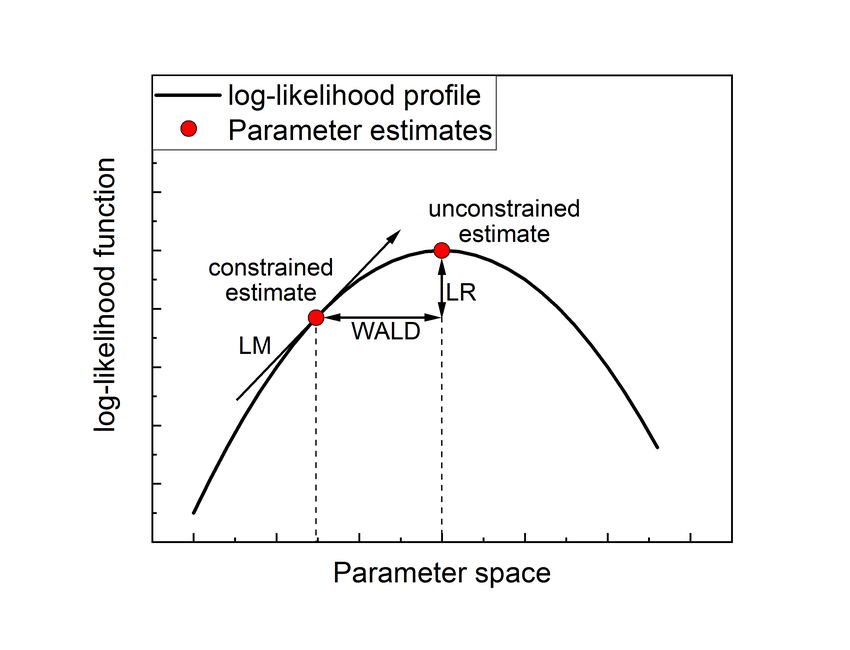
\includegraphics[height=\textheight]{./resources/lmlrwald.png}
\end{center}
\end{frame}

\begin{frame}{What to do in practice?}
\begin{itemize}
\item By reporting asymptotic standard errors you are implicitly using \alert{Wald} type statisitics.
\item If you are comparing models, you should probably try an \alert{LR} type statistic if you can.
\begin{itemize}
\item It used to be people didn't do this because $LR$ required maximizing the objective function more than once.
\item But computers today are pretty good...
\end{itemize}
\item For most extremum estimators (MLE, GMM, GEL, etc.) there are all three kinds of test-statistics
\begin{itemize}
\item ... and around the true $\theta_0$ as $N\rightarrow \infty$ they should coincide.
\item but in finite sample... anything can happen!
\end{itemize}

\end{itemize}

\end{frame}
\section*{Thanks!}

\end{document}